\documentclass{article}

% ------ TEMPLATE ------ %

% ---------------------- %

% ------ PACKAGES ------ %

\usepackage{charter}
\usepackage{geometry}
\usepackage{amsmath}
\usepackage{amssymb}
\usepackage{float}
\usepackage{graphicx}
\usepackage{tabularx}
\usepackage{array}
\usepackage{subcaption}
\usepackage{enumitem}
\usepackage{titlesec}
\usepackage{hyperref}
\usepackage{xcolor}
\usepackage{pifont}
\usepackage{fancyvrb}
\usepackage{listings}
\usepackage{multirow}
\usepackage{ulem}

% ---------------------- %

% ------ GENERALS ------ %

\setlist[itemize]{label=\scriptsize\textbullet}
\setlist[itemize]{noitemsep, topsep=1pt}
\setlist[enumerate]{noitemsep, topsep=1pt}

\titleformat{\chapter}[hang]
{\normalfont\huge\bfseries}{\thechapter}{1em}{}
\titleformat{\subsubsection}{\large\bfseries}{\thesubsubsection}{1em}{}

% ---------------------- %

% ------- COLORS ------- %

\hypersetup{
    colorlinks=true,
    linkcolor=blue!50!black,
    urlcolor=blue,
    citecolor=blue,
    pdfborder={0 0 0}
}

% ---------------------- %

% ------ COMMANDS ------ %

\newcommand{\vmark}{\textcolor{teal}{\ding{51}}}
\newcommand{\xmark}{\textcolor{red!70!black}{\ding{55}}}
\newcommand{\newpar}[0]{\vspace{2mm}\noindent}
\newcommand{\htitle}[1]{\newpar\textbf{#1 -}}
\newcommand{\ititle}[1]{\newpar\hspace{1em}\textbf{#1}}
\newcommand{\hyperlabel}[1]{\hypertarget{#1}\phantomsection\label{#1}}
\newcommand{\hyperitem}[2]{\item \hyperlink{#1}{#2}\leaders\hbox to 0.8em{\hss.\hss}\hfill\hbox to 1.8em{\hss\pageref{#1}}}
\newcommand{\stdtilde}[0]{\raise.17ex\hbox{$\scriptstyle\sim$}}
\newcommand{\xor}[0]{\char`\^}
\newcommand{\saveformula}[2]{\newbox{#1}\savebox{#1}{#2}}
\newcommand{\useformula}[1]{\usebox{#1}}

% ---------------------- %

\begin{document}

% -------- HEAD -------- %

\pagenumbering{gobble}

\begin{center}

    \fontsize{20pt}{30pt}\selectfont
    Well MEing

    \vspace{2cm}

    \fontsize{25pt}{45pt}\selectfont
    \textbf{Product Research Report}

    \vfill

    \fontsize{12pt}{18pt}\selectfont
    Matteo Bettiati \\
    Lorenzo Bianchi \\
    Alessio Caggiano \\
    Francesco Ostidich \\
    Denis Sanduleanu \\

    \vspace{1cm}

    \today \\
    \vspace{12pt}
    Version: 1.0
    \normalsize

\end{center}

\newpage
\pagenumbering{arabic}
\tableofcontents
\newpage

% ---------------------- %

% -------- BODY -------- %

\section{Introduction}

The purpose of this document is to present the research analysis behind the development of Well MEing, an application which aims to offer a highly customizable tracking system that allows users to define and monitor the well-being aspects that matter most to them.

\section{Market analysis}

\subsection{Overview of existing solutions}

In the applications stores, the Health \& Fitness category includes many sector-specific applications, such as Yazio for nutrition tracking, Strava for physical activity, and SleepTracker for sleep monitoring.
These apps focus on predefined tracking categories with specialized features, such as estimating calories from food photos.
However, they lack flexibility in adapting to users’ personalized wellness goals.

General tracking applications are not widely adopted.
Our analysis focused on three key apps in this space: HabitTracker, Habitify, HabitKit.

\subsection{Strengths and weaknesses of competitors}

Our competitive research highlights both the strengths and limitations of existing habit-tracking apps.
While some offer useful features, they also present significant drawbacks and gaps.

\begin{itemize}
    \item Limited customization options for habit tracking templates.
    \item Lack of efficient and general AI-based assistants for habit creation and progress tracking.
    \item Absence of voice interaction support.
    \item External device integration is missing in certain apps.
    \item Cluttered and unintuitive user interfaces, often overloaded with confusing elements.
\end{itemize}

These gaps present opportunities for improvement, particularly in enhancing personalization, AI-driven assistance, and user experience.

The following table presents an analysis of which features were available in the habit-tracking apps we tested.
These features closely align with those we afterwards included in the survey.

\begin{table}[H]
    \centering
    \begin{tabular}{l|c|c|c}
        \hline
        \textbf{Feature} & \textbf{HabitTracker} & \textbf{Habitify} & \textbf{HabitKit} \\
        \hline
        Flexible habit customization & \vmark \xmark & \vmark \xmark & \vmark \xmark \\
        AI-driven insights & \xmark & \xmark & \xmark \\
        Gamification elements & \vmark & \xmark & \vmark \\
        Voice-based logging & \xmark & \xmark & \xmark \\
        External devices support & \xmark & \vmark & \xmark \\
        Simple UI & \vmark & \vmark & \vmark \\
        Social community features & \vmark & \xmark & \xmark \\
        Notification for scheduled habit & \vmark & \vmark & \vmark \\
        \hline
    \end{tabular}
\end{table}

\section{User research}

\subsection{Research methodology}

To gather insights on user needs and expectations, we conducted a two-phase research process.

\begin{enumerate}
    \item \textbf{Structured survey}: we designed a Microsoft Forms survey with both closed-ended and open-ended questions to quantify user preferences. Key topics included: what aspects of well-being users would track, suggestions for improving habit-tracking apps, what would encourage continuous app usage.
    \item \textbf{Open-ended interviews}: we engaged users in guided conversations, using open-ended questions to explore their wellness habits and tracking preferences. While we had predefined topics, we encouraged participants to discuss unexpected concerns or needs that we might not have considered.
\end{enumerate}

We applied thematic analysis to process and interpret qualitative data.
This method involved systematically identifying, analyzing, and grouping recurring themes within user responses.
By coding open-ended answers and organizing them into meaningful patterns, we ensured that key insights emerged.

\subsubsection{Survey form}

To better understand user behavior, pain points, and expectations for a habit-tracking application, we conducted a survey that gathered more than 50 responses.

Alongside user-type questions like gender and age, we asked the following questions.

\begin{enumerate}
    \item Have you ever used an habit-tracking app before?
    \item If yes, which ones? And what would you change about this apps?
    \item If not, why? And what would make you use one of these apps?
    \item What would be useful to track for you?
    \item Which functionalities must not be missing?
    \item Do you have any idea suggestion?
\end{enumerate}

All the responses are collected in the tables found in the \hyperref[subsec:survey-responses]{Raw Survey Responses} section.

\subsubsection{Interview questions}

To gain deeper qualitative insights into user preferences and behaviors, we conducted a dozen interviews alongside the survey.

Even though the interviews were conducted in a colloquial manner, we tried to follow a predefined set of questions.

\begin{enumerate}
    \item Do you actively work on improving your well-being? If so, how?
    \item What metrics would you be interested in tracking?
    \item What were the shortcomings of similar apps you’ve used in the past, if any? If you’ve never used one, why?
    \item What innovative features would you like to see in an app of this kind?
    \item How could an app like this encourage you to use it consistently?
\end{enumerate}

The responses have been transcribed in the \hyperref[subsec:interview-responses]{Interview Responses Transcript} section.

\subsection{Results and analysis}

While the survey provided structured quantitative data, the interviews allowed for a more detailed exploration of user motivations, frustrations, and preferences.
This section presents the key findings from both approaches, highlighting recurring themes and user needs.

In the end, results were based on a diverse group of participants, with an even gender distribution and a wide range of ages.
The majority were between 20 and 30 years old, but other age groups were also well represented.

\subsubsection{Preferred habit categories}

To have a wider view of the application domain, we asked participants what kinds of habits they would be most interested in tracking.

\phantomsection\label{parag:stats-method}
The counting method we used first organizes structured form responses into predefined categories.
Then, each open-ended answer is analyzed, and the category’s count is increased whenever it is cited.
The responses revealed clear trends.

\begin{itemize}
    \item Physical Activity \& Fitness was the most common category, with people usually wanting to track step count and sport habits.
    \item Nutrition \& Hydration follows closely, including calories consumed and water drank.
    \item Health \& Wellness was also often cited, comprehending activities like sleep time, stress logging, medicine routines, skin care and heart beat rate monitoring.
    \item Productivity \& Time Management aspects, like study, hobby and work monitoring, or screen time, were also mentioned.
\end{itemize}

\begin{figure}[H]
    \centering
    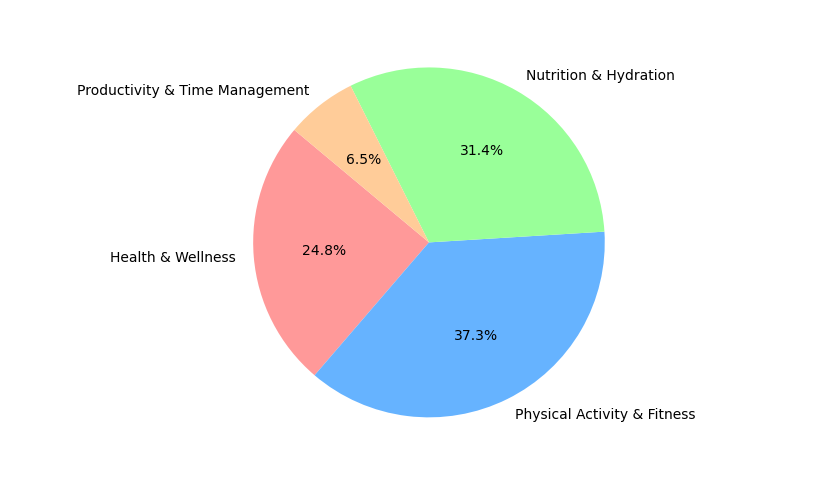
\includegraphics[width=0.6\textwidth]{images/tracked-categories.png}
\end{figure}

\subsubsection{Habit-tracking experience}

One of the first questions aimed to determine whether respondents had prior experience with habit-tracking applications.
More than 50\% of users had used at least one habit tracker before.

Many interviewees reported abandoning them due to several recurring pain points.

\begin{itemize}
    \item Tedious manual input: the requirement to log every detail was a sometimes a deterrent. Users favored automatic tracking.
    \item Excessive notifications: notifications are often excessive and should be easily toggled on or off.
    \item Lack of personalization: personalization is often seen as an important feature, since people tend to track similar things in different ways.
    \item Poor motivation mechanisms: many users lost interest due to the absence of engaging features, with some specifically pointing out a lack of gamification or social elements.
    \item Cluttered interface: overly complex or cluttered designs made navigation frustrating and unintuitive.
    \item Paid subscription: some users were unwilling to pay for essential features.
\end{itemize}

\subsubsection{Key user needs}

When asked what would encourage users to try and eventually use a habit-tracking app consistently, responses pointed to several recurring themes.
These findings confirm that users are looking for a highly flexible yet engaging experience, one that allows them to track their habits effortlessly while staying motivated through relevant feedbacks.

These statistics were collected with the \hyperref[parag:stats-method]{same method} we previously used.
From user responses, we found many critical aspects that should be fulfilled.

\begin{itemize}
    \item AI-driven insights, providing personalized habit suggestions and progress analysis, possibly science-based.
    \item Flexible habit customization, allowing users to define and modify what they track.
    \item Automated and voice-based logging, reducing manual effort and making tracking seamless.
    \item Tracking-devices integrations to reduce the need for redundant input.
    \item A highly customizable notification system, allowing users to tailor reminders based on preference and avoid unnecessary alerts.
    \item Gamification elements, such as streaks, challenges, and rewards, to maintain engagement.
    \item Social community features, enabling users to share progress, join group challenges, and support each other.
    \item A clean and intuitive UI, ensuring ease of use and an enjoyable experience.
\end{itemize}

\begin{figure}[H]
    \centering
    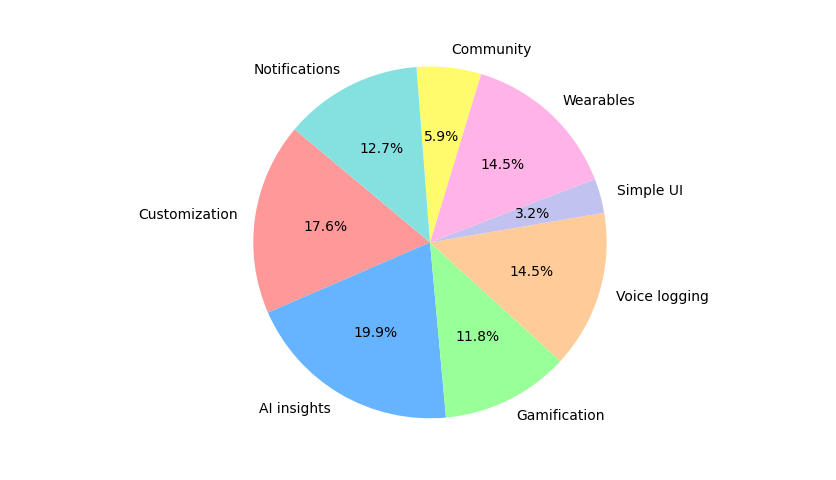
\includegraphics[width=0.6\textwidth]{images/user-aspects.png}
\end{figure}

\section{Feature prioritization}

\subsection{Methodology}

We applied a thematic analysis to survey responses, interviews, and market analysis to extract key insights about user needs and expectations for habit-tracking apps.
This method involves identifying, analyzing, and organizing patterns (themes) within the results found.

After gathering all data, we categorized features into thematic groups and ranked them based on their priority, which we determined mainly from the frequency of user mentions and the necessity which they expressed.
While our ranking primarily reflects user-driven priorities, we also lightly considered technical feasibility, which will be discussed in detail later.

We will now describe each category, list the features within them, and provide a ranked list of both categories and features.

\subsection{Categories description}

Based on our thematic analysis, we identified the following key categories, which we present and describe below.

\begin{enumerate}

    \item \textbf{Ease of use}: the app should be simple and intuitive to navigate, with a clean, visually appealing interface that feels engaging rather than cluttered. The input process should be quick and easy, minimizing the application learning curve. Voice-based input could enhance accessibility and speed up habit logging.

    \item \textbf{Personalization}: users highly value the ability to tailor their experience. This includes fully customizable and flexible habit tracking options without rigid templates. Personalized notifications and reminders should be adjustable based on user preference. Data visualization should be adaptable, offering multiple formats such as charts or diagrams.

    \item \textbf{AI insights}: AI-generated reports and recommendations should be integrated since users value insights (science-backed when possible) that evaluate their progress and optimize their habits. These insights should be provided at a set cadence.

    \item \textbf{User engagement}: to encourage non-committed users who do not have a strong necessity for habit-tracking, gamification and social features can help them stick with the app. Goal-setting options should also be available for those who need a target/objective to follow.

\end{enumerate}

\subsection{Ranked features list}

The table below presents the ranked list of features categorized by their respective themes.

\begin{table}[H]
    \centering
    \begin{tabularx}{0.9\textwidth}{c|X|X}
        \hline
        \textbf{Rank} & \textbf{Feature} & \textbf{Category} \\
        \hline
        1 & Custom habit creation & Personalization \\
        2 & Minimalistic UI & Ease of use \\
        3 & Quick habit logging & Ease of use \\
        4 & AI-generated progress reports & AI insights \\
        5 & Voice-based interaction & Ease of use \\
        6 & Targets & User engagement \\
        7 & Configurable notifications & Personalization \\
        8 & Adaptable data visualization & Personalization \\
        9 & Social interaction & User engagement \\
        10 & Game-like elements & User engagement \\
        \hline
    \end{tabularx}
\end{table}

\subsection{Features description}

Below we provide a short description for each feature.

\begin{enumerate}
    \item Users can define habits with custom names and tracking methods.
    \item User experience should be intuitive: each section of the app should contain few elements.
    \item Users can input habit progress with minimal steps.
    \item Users periodically receive a report containing progress analysis and suggestions.
    \item Users can input habit progress through voice commands.
    \item Users can define specific targets for each habit.
    \item Users can enable habit-specific reminders.
    \item Users can choose visualization formats (e.g. pie charts, progression bars).
    \item Users can commit to community leaderboards and shared progress tracking.
    \item Users can engage in a streaks, achievements and rewards system.
\end{enumerate}

\section{Technical feasibility}

\subsection{Paper for authoring tool}

This section reviews research papers which informed some of our implementation choices.
They helped us explore feasible approaches and potential limitations of the interaction automation functionalities we proposed.

GENO is a developer tool for authoring multimodal interaction on existing web applications.
It supports voice commands by invoking corresponding functions replaying GUI actions.
This approach highlights the importance of intent definition and event mapping within the graphical user interface (GUI), offering a structured method for speech-to-action integration.
For our implementation, we can leverage GENO’s approach for designing our system to map user voice commands to predefined actions utilizing existing interface elements.

OSTAAD is a multimodal system with memory for task automation.
It demonstrates how equipping systems with memory makes them capable of breaking down tasks into manageable steps for automating interactions, leveraging models like ChatGPT 4.0.
In general, using a memory component would allow the system to maintain context across interactions.

Another study, which analyzed cross-modality, AI-assisted prompt authoring, takes as example the ability of a model to generate code for producing ad-hoc graphs from user input.
It emphasizes on understanding the differences between spoken and written inputs, leading to more effective user interactions.

Implementing model-based interaction recognition agents with an high level of freedom through large language models (LLMs) like GPT-4 presents challenges due to their substantial resource requirements and development complexity.
In practice, these models often necessitate paid API access and may not consistently deliver the desired accuracy.

We propose utilizing pre-trained open-source models that, while having a lower capability level, could effectively map user interaction to a smaller set of fixed commands.

\subsection{Feasibility of features}

This section outlines how core functionalities can be structured to ensure a feasible implementation while maintaining a pleasing and efficient user experience.

\begin{itemize}

    \item Habit customization can be efficiently achieved through a predefined set of input fields, such as habit name, input type (e.g., integer, slider, rating, text), unit of measurement, and range constraints.
        Additionally, habits may be grouped into macro categories containing a set of tasks.
        This ensures full personalization to accommodate user needs for task tracking.

    \item To maintain a simple yet effective user interface, features can be organized into approximately five main sections, corresponding to app pages.
        For instance, these could include a main dashboard page for habit tasks and goals, a calendar/community section, an AI-related interactions page, a statistics section, and a user profile/notifications page.
        In general, the number of main features is sufficient to fully meet user needs while ensuring that the app’s design views remain intuitive and minimalistic.

    \item Incorporating a social community system introduces significant complexity in database structuring and authentication mechanisms, requiring multiple endpoints and design considerations.
        While not trivial to implement, it remains a feasible feature if its development effort is properly accounted for.
        Game-like features such as streaks, missions, and rewards are relatively easy to implement but still require careful consideration, particularly in UI design and, possibly, in AI-driven content generation.

\end{itemize}

\subsubsection{AI-based features}

This section explores the feasibility of AI-driven functionalities, focusing on natural language reports, voice-based interaction and a guided authoring tool, ensuring a balance between innovation and practical implementation.

\begin{itemize}

    \item AI-generated reports, presented in natural language and which can include habit summaries, analyze tracked data, and provide personalized suggestions for improvement, can be tailored to user-specific habits and past activity. Their feasibility depends on effective prompt engineering and could gain adaptive-precision possibly through fine-tuning a language model.

    \item A fully autonomous authoring tool may be impractical due to challenges in reaching a high accuracy. Furthermore, the environment in which it operates is a coding challenge itself, and security and reliability concearns are also difficult to fulfill.
        However, a guided system is feasible: the AI may map user input to a predefined set of functions with structured parameters, mirroring manual UI actions. This interaction would also work through speech-to-text conversion, leveraging built-in device capabilities for voice recognition. The AI would generate a preview of the requested actions, allowing the user to confirm execution.
        Given a good data set, the AI backbone could be enhanced by fine-tuning an open-source model to align its output with a desired format, which the software can easily interpret.

\end{itemize}

\subsection{Proposed technologies}

We think that the app should be designed specifically for mobile use, as the use condition mostly targets to fill short, idle time intervals, which are situations where users may be unlikely to open a web page.
A native mobile app can therefore be more suitable over a web-based approach.

For the frontend, we want to take Swift into consideration, as we think is the most suitable choice due to several advantages.

Its native performance ensures high responsiveness, and its UI components are visually appealing by default, reducing design effort.
Since iOS is widely adopted, Swift ensures better testing coverage granting also deeper features integration.
Being OS-specific, it moreover integrates well with voice recognition built-in functionalities, and seamlessly supports some wearable devices, aligning well with future development plans.
In general, since it is a modern and well-designed language, it simplifies development and deployment, while the alternatives are less appealing: React Native often results in buggy and imperfect interfaces, Flutter faces cross-compatibility challenges and limited adoption, and Kotlin, though viable, is Android-only, whereas iOS has broader user adoption.
Moreover, 80\% of the people we would engage for the testing phase have an iPhone.

For the backend, the choice of the language is flexible. For instance, Java or C\# are both viable, as they offer efficient and easy-to-use frameworks for APIs support.
The database selection is also open, with MySQL being a solid and widely supported option.

Regarding AI integration, the focus will primarily be on prompt engineering.
However, agreeing we find a good data set, model training is feasible using rental GPUs, which can offer enough resources for a possible fine-tuning leverage on pre-trained LLMs.

\newpage
\section{Appendix}

\subsection{Raw survey responses}
\label{subsec:survey-responses}

\begin{table}[H]
    \centering
    \begin{tabularx}{0.9\textwidth}{X|p{1in}}
        \hline
        \multicolumn{2}{l}{\textbf{Sex}} \\
        \hline
        Male & 30 \\
        \hline
        Female & 22 \\
        \hline
    \end{tabularx}
\end{table}

\begin{table}[H]
    \centering
    \begin{tabularx}{0.9\textwidth}{X|p{1in}}
        \hline
        \multicolumn{2}{l}{\textbf{Age}} \\
        \hline
        20- y.o. & 3 \\
        \hline
        20-40 y.o. & 40 \\
        \hline
        40-60 y.o. & 5 \\
        \hline
        60+ y.o. & 4 \\
        \hline
    \end{tabularx}
\end{table}

\begin{table}[H]
    \centering
    \begin{tabularx}{0.9\textwidth}{X|p{1in}}
        \hline
        \multicolumn{2}{l}{\textbf{Have you ever used an habit-tracking app before?}} \\
        \hline
        Yes & 28 \\
        \hline
        No & 24 \\
        \hline
    \end{tabularx}
\end{table}

\begin{table}[H]
    \centering
    \begin{tabularx}{0.9\textwidth}{X}
        \hline
        \textbf{If yes, which ones? And what would you change about this apps?} \\
        \hline
        I use an app to keep track of my running statistics. \\
        \hline
        Samsung Health, Apple Health \\
        \hline
        Zepp app \\
        \hline
        Daily steps, hours slept \\
        \hline
        I'd like more semplicity. \\
        \hline
        Sleep and vital parameters (when doing sport). Sleep-tracking-specific apps do not work well, even if associated with a smartwatch. \\
        \hline
        I use the Garmin watch, but I don't look often at its app. \\
        \hline
        Running \\
        \hline
        Clue app \\
        \hline
        Steps, burned calories \\
        \hline
        I use Apple Health, but I'd make it more interactive and I would add daily custom suggestions based on past data. I'd also add friends challenges to make users more willing to reach an objective (e.g. Who had taken the most steps this week?). \\
        \hline
        I use the Flo app. I'd track health, fitness and calories. \\
        \hline
        I'd like to have everything in a single app (sport, water, sleep, calories, steps...), with greater precision in counting. \\
        \hline
        I sometimes use Apple Health. \\
        \hline
        I'd like custom notifications about the many target I would set. \\
        \hline
        I use steps-counting apps. I'd like also a bluetooth compatibility. \\
        \hline
        I use apps to track calories assumptions and water drank. I would not change anything in these. \\
        \hline
        Steps tracking \\
        \hline
        I'd like non-invasive notifications. I'd like to be able to set which ones I desire. \\
        \hline
        I use health apps to visualize my daily steps: I would add the possibility to easily switch between steps and kilometers as measuring unit and to it would be nice being able to visualize both simultaneously. I also use a fun and playful app to track restroom breaks. \\
        \hline
        Apple Health is an example, but all these apps do not offer enough to make me get back every day; task are simple, and thus they rapidly become tedious and repetitive. There would be a way to make the experience more intriguing. \\
        \hline
        They're good enough, I would not change anything. \\
        \hline
        I track my diet. The only problem I see is that these apps often require paid subscriptions to unlock interesting features. \\
        \hline
        Samsung health. \\
        \hline
        I usually track Apple's statistics provided via the Apple Watch: i thus monitor my steps count, hearth rate and sleep time. I'd change the interface as it's not optimized therefore becoming dispersive. Fundamental things are not shown with ease. \\
        \hline
        Mi Fitness \\
        \hline
        I use MyFitnessPal to track calories of my meals and Sleep Cycle to monir my sleep. As for the first app, I'd change the insertion method, as it's too long and cumbersome; as for the second, I'd increase the number of parameters that could be tracked for the sleep. \\
        \hline
    \end{tabularx}
\end{table}

\begin{table}[H]
    \centering
    \begin{tabularx}{0.9\textwidth}{X}
        \hline
        \textbf{If not, why? And what would make you use one of these apps?} \\
        \hline
        I'm not constant enough, I'd rapidly stop using the app. \\
        \hline
        I have not enough will. \\
        \hline
        I've always seen these apps as a non-necessary addition. I distrust their effective utility: I do not think that they would be able to make the difference regarding how I want to regulate or monitor some aspects of my life/day. \\
        \hline
        For instance, I do not go to the gym, thus some aspects like heart beat monitoring would be useless to me. \\
        \hline
        No app really got my attention. Usually, I would download one for then deleting it the next day. \\
        \hline
        I'd like they would help me in my everyday life. \\
        \hline
        I don't have habits to track. \\
        \hline
        I'd use them, but I never found myself in the condition to do so. \\
        \hline
        Semplicity \\
        \hline
        Curiosity \\
        \hline
        They lack commodity, and I would suggest adding proofs of their effectiveness on my performances by displaying some concearning studies. \\
        \hline
        Objectives \\
        \hline
        An intuitive semplicity \\
        \hline
        Never had the necessity. \\
        \hline
    \end{tabularx}
\end{table}

\begin{table}[H]
    \centering
    \begin{tabularx}{0.9\textwidth}{X|p{1in}}
        \hline
        \multicolumn{2}{l}{\textbf{What would be useful to track for you?}} \\
        \hline
        Sleep time & 29 \\
        \hline
        Sport activities & 28 \\
        \hline
        Calories assumption & 26 \\
        \hline
        Daily steps & 22 \\
        \hline
        Heart rate & 17 \\
        \hline
        Water drank & 15 \\
        \hline
        Medicine consumption & 11 \\
        \hline
        Screen time & 1 \\
        \hline
        Skin care & 1 \\
        \hline
        Alcool/smoking & 1 \\
        \hline
        Study task and time & 1 \\
        \hline
        Stress & 1 \\
        \hline
        Hobby/work time & 1 \\
        \hline
    \end{tabularx}
\end{table}

\begin{table}[H]
    \centering
    \begin{tabularx}{0.9\textwidth}{X|p{1in}}
        \hline
        \multicolumn{2}{l}{\textbf{Which functionalities must not be missing?}} \\
        \hline
        Fully-customizable habits & 35 \\
        \hline
        Weekly/monthly report & 34 \\
        \hline
        External devices integration & 30 \\
        \hline
        Programmable habits with notifications & 24 \\
        \hline
        Game-like experience & 23 \\
        \hline
        Voice-based habit registration & 18 \\
        \hline
        Being able to follow other users and to have group-based habits & 11 \\
        \hline
        Voice-based habit creation & 8 \\
        \hline
        Intuitive and captivating interface & 1 \\
        \hline
        Pre-made habit templates/model from which to take inspiration & 1 \\
        \hline
    \end{tabularx}
\end{table}

\begin{table}[H]
    \centering
    \begin{tabularx}{0.9\textwidth}{X}
        \hline
        \textbf{Do you have any idea suggestion?} \\
        \hline
        Give feedback about the reached objectives. \\
        \hline
        App design and communication are to be customizable, for example, in terms of how the app motivates the user or responds to achieved and missed goals. Users could choose to make it more “sergeant-like” (strict, persistent, authoritative), For instance, in the case of someone who needs to take medication for health reasons but tends to underestimate its importance or forgets to take it. Alternatively, it could be more “friendly” (supportive, even in case of missed goals), for example, for someone trying to eat healthier or exercise but struggling and not wanting to feel additional pressure. Scientific and non-scientific anecdotes about the benefits the user would experience if they consistently reached their goals could also be integrated. \\
        \hline
        It should be very simple and fast to use. It is to be a way to keep track of everything the user want without having it to lose a lot of time. \\
        \hline
        These apps often require paid subscriptions to make more options available. This discourages the use of these apps in the first place. \\
        \hline
        Consider avoiding ads. \\
        \hline
        I've not found an app that is able to combine the alarm functionality with a vocal reminder for daily tasks. \\
        \hline
    \end{tabularx}
\end{table}

\subsection{Interview responses transcript}
\label{subsec:interview-responses}

\begin{enumerate}

    \item To improve my well-being, I try to reinforce positive behaviors: I eat healthy food, engage in beneficial activities, and observe how my body responds. The key metrics I would like to track include sleep, resting and effort-related heart rate (to assess stress impact), calorie intake, physical activity duration, time spent standing, and water consumption.
        Past experiences with similar apps have been frustrating due to unwanted reports or notifications; I prefer a more personalized approach. Ideally, an app should offer tailored reports and intelligently correlate data, such as how sleep quality is influenced by my physical activity. It should allow easy logging without feeling tedious and seamlessly integrate data across all my devices, including external app connections, so I don’t have to input everything manually.
        A crucial factor for consistent usage would be if my friends also used the app, but without forced challenges or streaks.

    \item I’m absolutely not committed to improving my well-being. Tracking calories is annoying because I have to input data; voice input would be better. I’d also be interested in tracking medications.
        I’ve never used similar apps because I never felt the need for them. If I were to use one, it should have an easy input method, giving less priority to gamification elements or social features showing what others do.
        My engagement wouldn’t depend on the app itself but rather on my personal need to track activities. However, having a visually appealing interface would make a difference.

    \item Yes, I focus on sports and nutrition. I’m interested in tracking calories and hours of exercise.
        I’ve used an app to track my workouts, but in general, I found access cumbersome and the information overload unhelpful.
        I’d like an app that calculates how many hours of exercise I need to stay fit, including necessary recovery time. It should tell me if my training makes sense: am I putting in enough effort? Do I need rest days? Am I walking at the right pace?
        I’d use the app if it works well and remains simple.

    \item I try a little, but I’m not really committed.
        I’d be interested in tracking nutrition, mostly by counting beers. Simple tracking like calorie intake and whether I followed my diet (yes/no) would be enough.
        What I found lacking in other apps was gamification and a sense of community (having a space to talk). I’ve used the HabitTracker, HabitKit and TickTick apps, but also other similar tools.
        Simplicity is key. I just need an easy way to input data, with minimal but well-designed elements. Gamification is important, similar to Duolingo.
        Streaks and gamification for input would be nice but not essential, as it’s a feature that may appeal a smaller target audience.

    \item I’ve used many health and fitness apps, but I always end up losing interest after a while. Most of them start out engaging, but they lack a strong motivation system to keep me coming back.
        I want an app that feels more like a game, with features such as streaks, daily missions, group challenges, and friendly competition, which would make it much more fun. If I could track progress alongside friends or compete in weekly challenges, I’d be much more likely to stick with it.
        The key is making it rewarding: unlocking achievements, leveling up, or even small animations when I reach a goal would help maintain engagement.

    \item I aim to maintain a balanced lifestyle but don’t track data obsessively. I’d like to monitor my overall physical activity, sleep quality, and stress levels without spending too much time inputting data.
        Previous apps I’ve tried were either too rigid or overloaded with unnecessary features. I’d prefer something adaptive that understands my habits over time and provides meaningful insights without bombarding me with notifications.
        A great addition would be contextual recommendations; for example, if my sleep worsens after intense workouts, the app could suggest better recovery strategies.

    \item I try to improve my well-being, but my motivation fluctuates. I’m interested in tracking hydration, screen time, and workout intensity, but only if inputting data is seamless.
        I stopped using other apps because they required too much manual input. I don’t want a tool that feels like extra work. Ideally, the app should automate as much as possible, maybe through sensors or integration with my smartwatch.
        I’d use it consistently if it provided insights that genuinely help me adjust my habits without overwhelming me with information.

    \item I’ve tried countless tracking apps, from step counters to full fitness suites, but I always end up quitting because they don’t push me to stay engaged. Simply logging data isn’t enough, I need something that makes the process exciting.
        I want a system with real incentives, like dynamic challenges, streak rewards, and interactive leaderboards. Maybe even collaborative goals where I team up with others to reach milestones.
        The app should make me feel like I’m progressing, not just logging numbers. If it felt more like a game, or in general something that gives me that sense of accomplishment, I’d definitely stick with it longer.

    \item My focus is on mental well-being rather than physical metrics. I’d be interested in tracking mood, stress levels, and time spent on relaxing activities.
        I avoid similar apps because they often focus too much on rigid goal-setting, which can feel discouraging. Instead, I’d like an app that adapts to my pace and provides encouraging nudges rather than unwanted strict targets.
        If the app helped me reflect on my progress in a non-judgmental way and provided small, manageable suggestions, I’d be more inclined to use it regularly.

    \item I don’t actively track my health, but I try to maintain a good routine. I’d consider monitoring heart rate, energy levels, and hydration if it didn’t require too much effort.
        I find most health apps overly structured, so that they feel like work rather than support. I’d appreciate an app that learns from my habits instead of forcing predefined routines.
        I’d be more engaged if the app occasionally provided science-backed insights about my progress rather than just numbers and graphs.

    \item I aim to be healthier but struggle with consistency. I’d like to track small lifestyle changes, such as steps taken, meal quality, and sleep trends.
        The biggest problem I’ve had with similar apps is the emphasis on perfection: if I miss a day, I don’t want to feel like I’ve failed. I prefer flexible tracking that allows me to adjust goals dynamically.
        If the app provided encouragement without making me feel guilty for setbacks, I’d be more likely to use it long-term.

    \item I mostly rely on intuition for my well-being but wouldn’t mind some structured tracking. I’d be interested in a minimalistic approach, tracking only a couple of key metrics, such as hydration and activity levels.
        I don’t use other apps because they feel too invasive. I don’t want something that constantly asks me to interact with it.
        I’d be more likely to use an app if it worked in the background, analyzed my habits passively, and provided occasional insights without requiring constant input.

\end{enumerate}

% ---------------------- %

\end{document}
